\chapter{Анализ предметной области} \label{chapt1}
\section{Типы индексов}
\subsubsection{B-Tree}
Самый популярный индекс, использующихся в большинстве СУБД как реляционных, так и нереляционных.
Существует много модификаций BTree: B+Tree (используется в CouchDB, MongoDB), SB-Tree (OrientDB).

Преимущества - логарифмическое время поиска, поддержка операций сравнения в запросах.

\subsubsection{Hash}
Следующий по популярности индекс. В запросах поддерживается только операция сравнения. В отличие от других вариантов хранится не само значение, а его хэш, что делает этот индекс компактным и быстрым.

\subsubsection{GiST (The Generalized Search Tree)}
Стратегия индексирования, основывающаяся на применении R-tree, RD-tree или B-tree. Предназначен для создания индексов по произвольным полям (для которых не поддерживается семантика сравнения и равенства в привычном смысле), при этом не важно, какую структуру имеют данные - одномерную или пространственную: геоданные, тексты, изображения и т.д.

Для каждого из этих типов данных должна быть определены поисковые и упорядочивающие операторы: принадлежность, содержание, совпадение, соответствие...

Подходит при большом количестве вставок и малом числе чтений.

Вместе с модификацией SP-GiST (Space Partitioning -- GiST) данный доступен в PostgreSQL.

\subsubsection{GIN (Generalized Inverted Index)}
Подобно GiST используется для индексирования произвольных полей.
Основная область применения --- полнотекстовый поиск. Другие примеры использования данного индекса: индексирование массивов, JSON, кроме этого PostgreSQL предоставляет довольно большое количество расширений для работы и с другими типами.

GIN-индексы хороши своей компактностью. Недостатком данного индекса является медленная вставка и обновление данных.

\subsubsection{Inverted index}
Индекс, использующаяся для полнотекстового поиска. Содержит список слов и документов, в которых оно встретилось.

Полнотекстовые запросы выполняют лингвистический поиск в текстовых данных путем обработки слов и фраз в соответствии с правилами конкретного языка.

Реализации полнотекстового поиска варьируются в различных СУБД. Инвертированный индекс используется в Microsoft SQL Server, MySQL, OrientDB и поисковом движке Elasticsearch.

\subsection{Пространственные индексы}
Большинство современных СУБД имеют типы, предназначенные для работы с пространственными типами данных: точки, прямые, окружности и другие геометрические объекты. Для данных объектов используются свои стратегии индексирования.

Известными решениями является использование пространственной сетки (spatial grid), дерева квадрантов (quadtree) и R-Tree.

Данные индексы используются графовыми базами данных (Neo4j, AllegroGrath), однако существуют специальные дополнения и расширения, основанные на известных СУБД, но предназначенные для обработки исключительно пространственной информации - PostGIS, Oracle Spatial, GeoAPI в Redis.

\subsubsection{R-Tree}
Подходит для поиска объектов в 2-3--мерном пространстве. Идея лежащая в основе индекса --- группировка объектов в зависимости от расстояния друг до друга. Это ускоряет поиск, однако происходит потеря точности, и возвращенный результат может не быть абсолютно точным.

Существует несколько модификаций R-Tree: R+-Tree, R*-Tree. Обобщением R-Tree является X-Tree, который позволяет индексировать данные произвольных размерностей.

Данный тип индекса поддерживается некоторыми движками СУБД MariaDB (SPATIAL INDEX), PostgreSQL (RTREE), Oracle.

\subsubsection{UB-Tree (Universal B-Tree)}
Индекс используемый для хранения многомерных данных в одномерной структуре. К каждому значению применяется преобразование Мортона, заключающееся в чередовании двоичных цифр координатных значений, полученный результат называется Z-последовательностью (Z-order curve). Для обработки одномерных данных используется обычное B-дерево.

\begin{figure}[ht] 
	\centering
	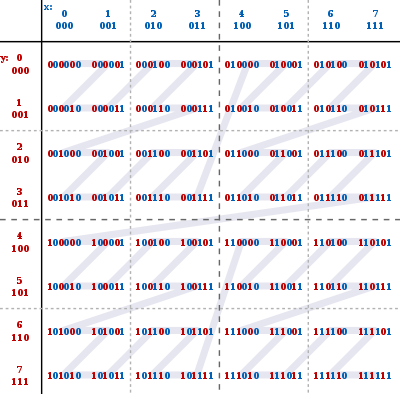
\includegraphics [scale=0.5] {zcurve2d}
	\caption{Построение Z-последовательности}
	\label{img:zcurve2d}
\end{figure}

Позволяет эффективно производить поиск по интервалам значений, однако часть возвращаемого результата может и не находиться в указанном интервале (рис.~\ref{img:zcurve2d_interval}), поэтому при запросе приходится применять дополнительные механизмы для фильтрации данных. Это накладывает некоторые ограничения на целесообразность применения данного индекса. Запросы должны быть.

\begin{itemize}
	\item \textbf{Часто задаваемыми}. Распространена практика, когда часть параметров запроса не задается, а остается открытой, однако в данном случае это может серьезно влиять на производительность.
	\item \textbf{<<Избирательным>>}. Границы, устанавливаемые при запросе должны исключать большие объемы данных. Для неравномерно распределенных логических значений пространство поиска может быть сильно увеличено.
\end{itemize}

\begin{figure}[ht] 
	\centering
	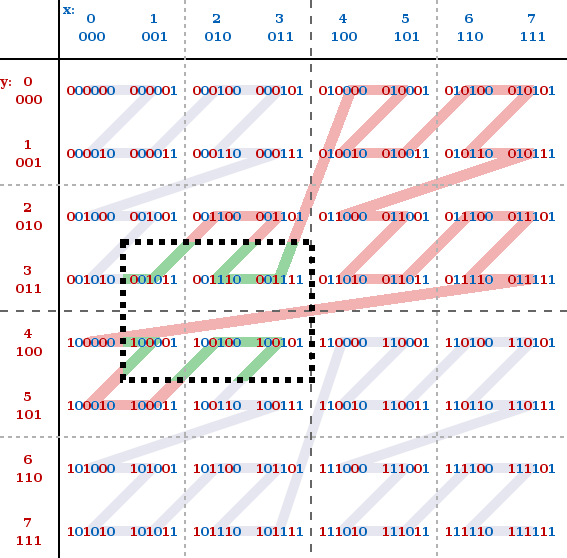
\includegraphics [scale=0.35] {zcurve2d_interval}
	\caption{Поиск значений в интервале}
	\label{img:zcurve2d_interval}
\end{figure}

При реализации Z-адрес рассматривается исключительно как битовая последовательность. Это значит, что единственное ограничение на тип ключа --- возможность упорядочивания при переходе к двоичному представлению. В итоге доступные типы ограничиваются не только целыми числами, но и числами с плавающей точкой, строками, временными метками...

Данный тип индексирование используется в TransBase\cite{ramsak2000integrating}, Accumulo, HBase \cite{nishimura2011md}, DynamoDB\cite{DynamoZorderP1, DynamoZorderP2}. 

Стоит отметить, что данное преобразование не является единственным для отображения многомерных данных в одномерные. Могут использоваться кривые Гильберта или Пеано. Однако Z-последовательность гораздо проще для вычисления.

\subsection{Индексы c использованием машинного обучения}
Можно выделить несколько подходов, которые могут быть использованы для поиска информации и выделения закономерностей в больших массивах данных --- Latent Semantic Indexing (LSI) и Hidden Markov Model (HMM). Данные варианты хоть и являются интересными и полезными в некоторых сферах, но примеров их использования в каких--либо СУБД нет.

\section{Используемые индексы в различных СУБД}
\begin{tabular}{|c|c|{c}}
	\hline
	СУБД & Индексы\\
	\hline
	PostgreSQL & B-Tree, R-Tree, Hash, GiST,\\ 
	& SP-GiST, GIN, RUM, BRIN, Bloom  \\
	MySQL/MariaDB & B-Tree, Hash, R-Tree, Inverted Index  \\
	Oracle &  B-Tree, B-Tree--cluster,\\
	& Hash--cluster, Reverse key, Bitmap\\
	MongoDB & B-Tree, Geohash, Text index, Hash \\
	OrientDB & SB-Tree, Hash, Lucene Fulltext, Lucene Spatial \\
	MemSQL & SkipList, Hash, Columnstore \\ \hline
\end{tabular}